%%%%%%%%%%%%%%%%%%%%%%%%%%%%%%%%%%%%%%%%%
% Beamer Presentation
% LaTeX Template
% Version 1.0 (10/11/12)
%
% This template has been downloaded from:
% http://www.LaTeXTemplates.com
%
% License:
% CC BY-NC-SA 3.0 (http://creativecommons.org/licenses/by-nc-sa/3.0/)
%
%%%%%%%%%%%%%%%%%%%%%%%%%%%%%%%%%%%%%%%%%

%----------------------------------------------------------------------------------------
%	PACKAGES AND THEMES
%----------------------------------------------------------------------------------------

\documentclass{beamer}
\usepackage{amsmath, amssymb}

\usepackage{bm}

\mode<presentation> {

% The Beamer class comes with a number of default slide themes
% which change the colors and layouts of slides. Below this is a list
% of all the themes, uncomment each in turn to see what they look like.

%\usetheme{default}
%\usetheme{AnnArbor}
%\usetheme{Antibes}
%\usetheme{Bergen}
%\usetheme{Berkeley}
%\usetheme{Berlin}
%\usetheme{Boadilla}
%\usetheme{CambridgeUS}
%\usetheme{Copenhagen}
%\usetheme{Darmstadt}
%\usetheme{Dresden}
%\usetheme{Frankfurt}
%\usetheme{Goettingen}
%\usetheme{Hannover}
%\usetheme{Ilmenau}
%\usetheme{JuanLesPins}
%\usetheme{Luebeck}
\usetheme{Madrid}
%\usetheme{Malmoe}
%\usetheme{Marburg}
%\usetheme{Montpellier}
%\usetheme{PaloAlto}
%\usetheme{Pittsburgh}
%\usetheme{Rochester}
%\usetheme{Singapore}
%\usetheme{Szeged}
%\usetheme{Warsaw}

% As well as themes, the Beamer class has a number of color themes
% for any slide theme. Uncomment each of these in turn to see how it
% changes the colors of your current slide theme.

%\usecolortheme{albatross}
%\usecolortheme{beaver}
%\usecolortheme{beetle}
%\usecolortheme{crane}
%\usecolortheme{dolphin}
%\usecolortheme{dove}
%\usecolortheme{fly}
%\usecolortheme{lily}
%\usecolortheme{orchid}
%\usecolortheme{rose}
%\usecolortheme{seagull}
%\usecolortheme{seahorse}
%\usecolortheme{whale}
%\usecolortheme{wolverine}

%\setbeamertemplate{footline} % To remove the footer line in all slides uncomment this line
%\setbeamertemplate{footline}[page number] % To replace the footer line in all slides with a simple slide count uncomment this line

%\setbeamertemplate{navigation symbols}{} % To remove the navigation symbols from the bottom of all slides uncomment this line
}

\usepackage{graphicx} % Allows including images
\usepackage{booktabs} % Allows the use of \toprule, \midrule and \bottomrule in tables

%----------------------------------------------------------------------------------------
%	TITLE PAGE
%----------------------------------------------------------------------------------------

\title[GCWM]{Modeling Frequency and Severity of Claims with the Generalized Cluster-Weighted Model } % The short title appears at the bottom of every slide, the full title is only on the title page

\author{Nik Po\v cu\v ca} % Your name
\institute[McMaster University] % Your institution as it will appear on the bottom of every slide, may be shorthand to save space
{
McMaster University \\ % Your institution for the title page
\medskip
\textit{Tatjana Miljkovic, Petar Jevti\' c, and Paul McNicholas} % Your email address
}
\date{\today} % Date, can be changed to a custom date

\begin{document}

\begin{frame}
\titlepage % Print the title page as the first slide
\end{frame}

\begin{frame}
\frametitle{Overview} % Table of contents slide, comment this block out to remove it
\tableofcontents % Throughout your presentation, if you choose to use \section{} and \subsection{} commands, these will automatically be printed on this slide as an overview of your presentation
\end{frame}

%----------------------------------------------------------------------------------------
%	PRESENTATION SLIDES
%----------------------------------------------------------------------------------------

%------------------------------------------------
\section{Heterogeneity of Risk} % Sections can be created in order to organize your presentation into discrete blocks, all sections and subsections are automatically printed in the table of contents as an overview of the talk
%------------------------------------------------

\begin{frame}
\frametitle{Introduction to Risk}
Sub-grouping of insurance policies based on risk classification is a standard practice in insurance. The heterogenous nature of insurance data allows for explorations of many different techniques for sub-grouping risk. As a result, there is a growing number of papers in the area of mixture modeling of univariate and multivariate insurance data to account for heterogeneity of risk. 
\\~\\
\end{frame}
%------------------------------------------------
\begin{frame}
\frametitle{Examples in Insurance}
\begin{block}{Automotive}
Drivers of various levels of competency are mixed in with large groups rates and are often difficult to track within a cohort. 
\end{block}
\begin{block}{Health/Life}
The variance among people's lifestyles tend to dictate their life expectancy as well as healthcare coverage. Again how do you define a ``lifestyle" in a quantitative sense?
\end{block}
\begin{block}{Maritime}
Maritime Surveillance Radar data is often used to price maritime insurance which have had  success being modelled as a mixture of distributions. 
\end{block}
\end{frame}

%------------------------------------------------

\section{Cluster Weighted Models}


\begin{frame}
\frametitle{Cluster Weighted Models}
Let $(\bm{X^{'}}, Y)^{'}$  be the pair of a vector of covariates  $\bm{X}$ and a response variable $Y$. Assume this set is defined on some sample space $\Omega$ that takes values in an appropriate Euclidian subspace. Furthermore, assume that there exists $G$ partitions of $\Omega$, denoted as $\Omega_1, \ldots, \Omega_G$. \newline

Gershenfeld (1997) characterized the cluster-weighted models as a finite mixture of GLMs hence, the joint distribution $f(\bm x, y)$ of $(\bm{X^{'}}, Y )^{'}$  is expressed as follows
 \begin{align}
 f(\bm x, y)= \sum_{j=1}^{G} \tau_j q(y|\bm{x};\Omega_j)p(\bm{x};\Omega_j).
\label{eq1}
\end{align}
\\~\\
\end{frame}

%------------------------------------------------
\begin{frame}
\frametitle{Extending CWM}
(Ingrassia, Punzo et. al. 2015) proposed a flexible family of mixture models for fitting the joint distribution of a random vector $(\bm{X^{'}}, Y)^{'}$ by splitting the covariates into continuous and discrete as $ \bm{X}=(\bm{V^{'}},  \bm{W^{'}})^{'}$.

\begin{align*}
 f(\bm{x}, y; \bm{\Phi})= \sum_{j=1}^{G} \tau_j q(y|\bm{x};\bm{\vartheta}_j)p(\bm{x};\bm{\theta}_j)\\ 
= \sum_{j=1}^{G} \tau_j q(y|\bm{x};\bm{\vartheta}_j)p(\bm{v}; \bm{\theta}_j^{\star})p(\bm{w};\bm{\theta}_j^{\star\star})
 \end{align*}
\end{frame}

%------------------------------------------------

\section{Generalizing CWM}
\begin{frame}
\frametitle{Generalizing CWM}
We proceed to extend CWM by splitting the  continuous covariates further as $\bm{V}:=(\bm U^{'}, \bm T^{'})^{'}$, where $\bm{U}$ is a set of non-Gaussian covariates, and $\bm{T}$ a set of Gaussian  covariates.  Thus CWM is now recovered as
\begin{align*}
 f(\bm x, y; \bm{\Phi})= \sum_{j=1}^{G} \tau_j q(y|\bm{x};\bm{\vartheta}_j)p(\bm{t};\bm{\theta}_j^{\star})p(\bm{w};\bm{\theta}_j^{\star\star})p(\bm{u};\bm{\theta}_j^{\star\star\star})
\end{align*}
\end{frame}


%------------------------------------------------

\begin{frame}
\frametitle{Non-Gaussian Covariate}
With a log-normal assumption for $p(\bm{u};\bm{\theta}_j^{\star\star\star})$ we have that $\bm{u}$ is defined on $\mathbb{R}^p_+,\quad p \in \mathcal{N}$ with parameter vector $ \bm{\theta}_j^{\star\star\star} $ having probability density function as
\begin{small}
$$ 
p \left(  \bm{u}; \bm{\theta}_j^{\star\star\star} := ( \bm{\mu}_j^{\star\star\star} ,\bm{ \Sigma}_j^{\star\star\star } ) \right)
$$
$$ 
= \frac{1}{(\prod_{i=1}^{p}u_{i})|\bm{ \Sigma}_j^{\star\star\star} |(2 \pi)^{\frac{p}{2}}}   \exp\left[-\frac{1}{2}(\ln\bm{ u}-\bm{\mu}_j^{\star\star\star})^{'}\bm{\Sigma}_j^{{\star\star\star}_{-1}}(\ln \bm {u}-\bm{\mu}_j^{\star\star\star})\right].
$$
\begin{itemize}
\item Extreme Weather Events
\item Population Density
\end{itemize}
\end{small}
\end{frame}
%------------------------------------------------
\begin{frame}
\frametitle{Zero - Inflated Poisson}
\begin{small}
Made famous by Lambert (1992), the zero -inflated Poisson model accounts for the presence of excess zeros in data. 
 \begin{align*}
 f(\bm x, y; \Phi)= \sum_{j=1}^{G} \tau_j \left[ q(y = 0|\bm{x};\bm{\vartheta}_{j} ) +  q(y > 0|\bm{x} ; \bm{\vartheta}_{j}  ) \right]   p(\bm{t};\bm{\theta}_j^{\star})p(\bm{w};\bm{\theta}_j^{\star\star})p(\bm{u};\bm{\theta}_j^{\star\star\star}). \\
\end{align*}
\end{small}
\end{frame} 
%------------------------------------------------
\section{Zero - Inflated Poisson}
\newcommand{\xTilda}{\bm{\tilde{x}}}
\begin{frame}
\frametitle{Zero - Inflated Poisson}
$$ 
 q( y = 0| \bm{x} ; \bm{ \vartheta}_{j}  ) = \psi_j + (1 - \psi_j)e^{-\lambda_j},
$$

$$ 
q(y > 0 |  \bm{x} ; \bm{ \vartheta}_{j}  ) = (1 - \psi_j)e^{-\lambda_j} \frac{\left(\lambda_j \right)^y  }{y!}.
 $$
$$
 \psi_j =  \frac{e^{\xTilda \bm{\bar{\beta}}_j'}}{1+ e^{\xTilda \bm{\bar{\beta}}_j'}}   \quad \quad \quad
\lambda_j  = e^{\xTilda \bm{\beta}_j'}. 
$$
\end{frame} 

%------------------------------------------------
\begin{frame}
\frametitle{Bernoulli-Poisson Partitioning Method}
\begin{small}

 \begin{align*}
\Omega^B =  \bigcup_{l =1}^G \Omega_l^B & & &  &
f^B(\bm x, y; \Phi)= \sum_{l=1}^{G} \tau_l q^B(y|\bm{x}; \bm{\bar{\beta}}_l) p(\bm{t};\bm{\theta}_l^{\star})p(\bm{w};\bm{\theta}_l^{\star\star})p(\bm{u};\bm{\theta}_l^{\star\star\star}).
\end{align*}
$$
 \psi_l =  \frac{e^{\xTilda \bm{\bar{\beta}}_l'}}{1+ e^{\xTilda  \bm{\bar{\beta}}_l'}}  \quad \quad \quad
 q^B(y | \bm{x} ;  \bm{\bar{\beta}}_l) = \begin{cases}
      \quad \psi_l, & y = 0\\
     1 -  \psi_l,  & y > 0
   \end{cases} 
$$
\begin{align*}
\Omega^P =  \bigcup_{j =1}^M \Omega_j^P & &  &  &
f^P(\bm x, y; \Phi)= \sum_{j=1}^{M} \tau_j q^P(y|\bm{x};\bm{\beta}_{j}) p(\bm{t};\bm{\theta}_j^{\star})p(\bm{w};\bm{\theta}_j^{\star\star})p(\bm{u};\bm{\theta}_j^{\star\star\star}).
\end{align*}
 \begin{align*}
\lambda_j = e^{\xTilda \bm{\beta}_j'}, & & & & %\beta_{0j} + \beta_j^{'}x
q^P(y|\bm{ x} ; \lambda_{j} ) = e^{-\lambda_j} \frac{{\lambda_j}^y}{y!}.
 \end{align*}
\end{small}
\end{frame}
%------------------------------------------------
\section{EM Algorithm for Estimation}
\begin{frame}
\frametitle{Bernoulli-Poisson Partitioning Method}
$$\Omega =  \Omega^Z = \bigcup_{ \substack {l \in \{1 ,\ldots, G \} \\ j \in \{1 ,\ldots, M \}}  } \Omega_{l,j}^Z := \bigcup_{\substack{ l \in \{1 ,\ldots, G \} \\ j \in \{1 ,\ldots, M \}  } }  \Omega_l^B \cap \Omega_j^P =: \bigcup_{k \in \{1 ,\ldots, K\leq M \times G \}} \Omega_k^Z, $$
\begin{small}
$$q^Z_{k}(y|\bm{x};  \bm{\bar{\beta}}_k,\bm{ \beta}_k)  := q^B(y|\bm{x}; \bm{\bar{\beta}}_k) +(1-  q^B(y|\bm{x}; \bm{\bar{\beta}}_k) ) q^P(y|\bm{x};\bm{\beta}_k) $$
 $$ = q(y = 0|\bm{x};\bm{\vartheta}_{k} ) +  q(y > 0|\bm{x} ; \bm{\vartheta}_{k}), \quad k \in \{1 ,\ldots, K \}. $$
 
\end{small}
\end{frame}
%------------------------------------------------
\begin{frame}
\frametitle{EM  Algorithm for CWM (Ingrassia et al, 2016)}
\underline{E-Step}
\begin{tiny}
\begin{equation*}\begin{split}
    {\pi_{ij}}^{(s)} &= {E}[Z_{ij} |(\bm{x_i}, y_i); \bm{\Phi}^{(s)}]\\
     &= \frac{{\tau_j}^{(s)}q(y_i|x_i; \bm \beta_j^{(s)}, \lambda^{(s)}_{j})p(t_i; \bm\mu_j^{{\star}(s)}, \bm\Sigma_j^{{\star}(s)}) p(w_i; \bm \gamma_j^{(s)})p(u_i; \bm{\mu}_j^{\star\star\star (s)},\bm{\Sigma}_j^{\star\star\star (s)})}{f(\bm{x}_i, y_i; \bm{\Phi}^{(s)})
\label{eq29}                       }.
\end{split}\end{equation*}
\end{tiny}
\underline{M-Step}
\begin{tiny}
\begin{align*}
{\hat{\tau}_j}^{(s+1)}&=\frac{1}{n} \sum_{i=1}^n \pi_{ij}^{(s)}, && && {\hat{\bm{\mu}}_j}^{\star (s+1)}=\frac{1}{\sum_{i=1}^n \pi_{ij}^{(s)}} \sum_{i=1}^n \pi_{ij}^{(s)}\bm t_i, &&  && {\hat{\bm \gamma}^{(s+1)}_{jr}} =\frac{\sum_{i=1}^n \pi_{ij}^{(s)} \omega^{rs}_i} {\sum_{i=1}^n \pi_{ij}^{(s)}},
\end{align*}
$$
 {\widehat{\bm \Sigma^{}}_j}^{\star(s+1)}=\frac{1}{\sum_{i=1}^n \pi_{ij}^{(s)}} \sum_{i=1}^n \pi_{ij}^{(s)}(\bm t_i-\hat{\bm \mu}^{(s+1)}_j) (\bm t_i-\hat{\bm \mu}^{(s+1)}_j)^{'}  ,
$$
\end{tiny}
\end{frame}
%------------------------------------------------
\begin{frame}
\frametitle{M-Step for Log-normal}
\begin{small}
\begin{align*}
{\hat{\bm \mu}_j}^{\star\star\star (s+1)} &=\frac{1}{\sum_{i=1}^n \pi_{ij}^{(s)}} \sum_{i=1}^n \pi_{ij}^{(s)}\ln \bm u_i, \\
{\widehat{\bm \Sigma}_j}^{\star\star\star(s+1)} & =\frac{1}{\sum_{i=1}^n \pi_{ij}^{(s)}} \sum_{i=1}^n \pi_{ij}^{(s)}(\ln \bm u_i-\hat{\bm \mu}^{\star\star\star(s+1)}_j) (\ln \bm u_i-\hat{\bm \mu}^{\star\star\star(s+1)}_j)^{'}. 
\end{align*}
\end{small}
\end{frame}
%------------------------------------------------
\begin{frame}
\frametitle{EM  Algorithm for Zero-Inflated (Lambert, 1992)}
\begin{center}
\underline{E - Step}
\end{center}
\begin{small}
\begin{align*}
o_{ik}^{(s)} = \begin{cases}  \left[ 1 + \exp{\big(-\xTilda_i \bar{\bm{\beta}_k}^{'(s)} - e^ {\bm{\xTilda_i} \bm{\beta}_k^{'(s)}} \big) } \right]^{-1}, &  y_{i} = 0 \\
  0 \quad , & y_{i}> 0 .
\end{cases}
\end{align*}
\end{small}

\begin{center}
\underline{M - Step}
\end{center}
\begin{small}
\begin{align}
 l_c(\lambda_k; y,\bm{x},\bm{o}_k^{(s)}) &= \sum_{i=1}^n (1- o_{ik}^{(s)}) (y_i \xTilda_i \bm{\beta}_k^{'}  - e^{\xTilda_i \bm{\beta}_k^{'}})\label{eq7}.\\
l_c(\psi_k;y,\bm{x},\bm{o}_k^{(s)}) &=\sum_{i=1}^n \left( o_{ik}^{(s)} \xTilda_i \bar{\bm{\beta}_k }^{'} - \log \left(1+ e^{ \xTilda_i \bar{\bm{\beta}_k }^{'}} \right) \right), \label{eq6}   
 \end{align}
\end{small}
\end{frame}
%------------------------------------------------
\section{Comparison of Models}
\begin{frame}
\frametitle{Comparison of Models}
How do we know which model is the best, the zero-inflated or standard Poisson? (Wilson, 2016) demostrates the misuse of the Vuong non-nested t-test (Vuong, 1984). Wilson instead defines a replacement in the form of a LR test. 
\begin{align*}
& & H_0: \quad \psi_k = 0 \quad\quad vs. \quad\quad H_a: \quad \psi_k \neq 0 . & &
\end{align*}
\begin{center}The test statistic $\varphi$ is defined as \end{center}
\begin{align}
\varphi = -2 \bigg[l(\tilde{\lambda_k}; y, \bm{x}) - l(\lambda_k, \psi_k; y , \bm{x} )\bigg].
\end{align}
\end{frame}

\section{Application}
\begin{frame}
\frametitle{Application - French Motor Policy}
A collection of insurance policy information pertaining to motorists in all 24 regions of France. The dataset is loaded from the CASDatasets package (Dutang, 2014). 
\begin{small}
\begin{table}[!htb]
\begin{center}
      \centering
        \begin{tabular}{ll}
\hline
Attribute & Description \\
\hline
Policy ID & Unique identifier of the policy holder\\
Claim Nb & Number of claims during exposure period  (0,1,2,3,4)\\
Exposure & The exposure of policy in years (0--1.5) \\
Power & Power level of car ordered categorical (12 levels )\\
Car Age & Car age in years \\
Driver Age & Age of a legal driver \\
Brand & Car brands (7 types) \\
Gas & Diesel or Regular \\
Region & Regions in France (10 classifications)\\
Density & Number of inhabitants per km$^2$ \\
Loss Amount & Portion of claim the insurance policy pays\\
\hline
		\end{tabular}
\end{center}
\end{table}
\end{small}
\end{frame}

%------------------------------------------------
\begin{frame}
\frametitle{Modelling Severity}
$$ Loss Amount =  Density + Car Age + Driver Age + Region + Power + Gas + \epsilon, \quad $$
$$ 
\epsilon \sim \mathcal{N}(0,\sigma^2). 
$$ \newline
The canonnical log-link is used for the GLM. The
$CarAge$ is modelled as a categorical variable with five categories: $[0,1)$, $[1,5)$, $[5,10)$, $[10,15)$, and $15+$. Additionally, $DriverAge$ is modelled as a categorical variable with five categories: $[18,23)$, $[23,27)$, $[27,43)$, $[43,75)$, and $75+$. $Power$ is modelled into three categories as in (Charpentier ,2014).

\end{frame}
%------------------------------------------------
\begin{frame}
\frametitle{Comparison of GCWM to CWM}
\begin{center}
\begin{tabular}{@{\extracolsep{5pt}} rrrr}
\\[-1.8ex]\hline
\hline \\[-1.8ex]
Model & k & AIC & BIC \\
\hline \\[-1.8ex]
CWM & $1$ & $$$352,470$ & $$$352,661$ \\
& $2$ & $$$314,560$ & $$$314,949$ \\
& $3$ & $$$301,223$ & $$$301,812$ \\
& $4$ & $$$287,020$ & $$$287,808$ \\
& $\bm{5}$ &$$$\bm{284,283}$ & $$$\bm{285,268}$ \\
GCWM & $1$ & $$$111,129$ & $$$111,320$ \\
& $2$ & $$$90,039$ & $$$90,428$ \\
& $3$ & $$$89,476$ & $$$90,065$ \\
& $\bm{4}$ & $$$\bm{88,781}$ & $$$\bm{89,568}$ \\
& $5$ & $$$88,731$ & $$ $89,717$ \\
\hline \\[-1.8ex]
\end{tabular}
\end{center}
\end{frame}
%------------------------------------------------

\begin{frame}
\frametitle{Modelling Severity}
\begin{figure}[!htb]
\label{fig:vet1}
\begin{center}
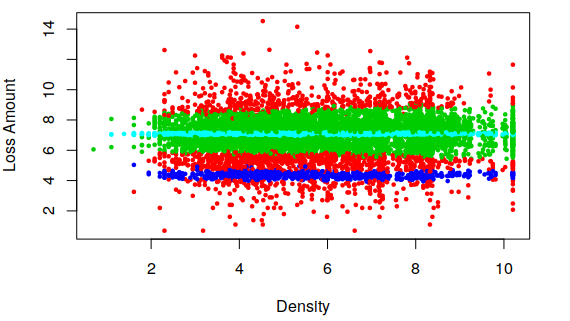
\includegraphics[scale=0.83]{SeverityPlot}
\end{center}
\end{figure}
\end{frame}

%------------------------------------------------
\begin{frame}
\frametitle{Volatility Clusters}
\begin{tabular}{rrrrrr}
\hline\hline
Volatility Level - (Cluster)  $\quad$    & Minimum & Mean  & Maximum & $\sigma$    \\
\hline
V1 - (3)$\quad\quad\quad$ & 51  & 79 & 154 & \textbf{ 13} \\
V2 - (4)$\quad\quad\quad$ & 1,039  & 1,109  &  1,324 & \textbf{ 52} \\
V3 - (2)$\quad\quad\quad$ & 221 & 1,687  & 8,841  &\textbf{ 1,284}  \\
V4 - (1)$\quad\quad\quad$ & 2 & 9,717 & 2,036,833  & \textbf{ 64,835}   \\
\hline\hline
\end{tabular}
\end{frame}
%------------------------------------------------
\begin{frame}
\frametitle{Modelling Frequency}
\begin{equation}
Claim Nb = Density + Exposure + Power \quad|\quad Exposure + Car Age
\end{equation}
\end{frame}

%------------------------------------------------
\begin{frame}
\frametitle{Frequency Plot}
\begin{center}
\label{frequencyGraph}
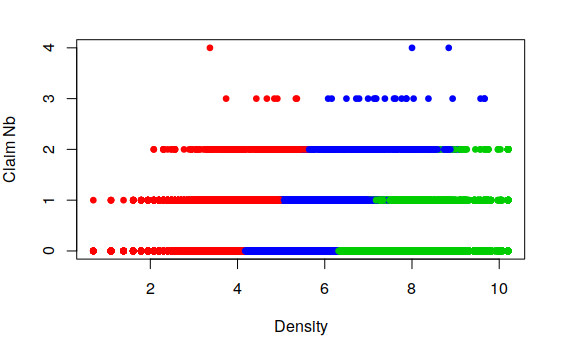
\includegraphics[scale=0.80]{frequency.png}
\end{center}
\end{frame}


%------------------------------------------------
\begin{frame}
\frametitle{Density Clusters}
\begin{center}
\begin{tabular}{rrrrrr}
\hline
\hline
Cluster  & Color & Minimum & Mean & Maximum & $\sigma$  \\
\hline
1 &   Red         & 0.69    & 3.38 & 5.60    & 0.60  \\
2 &  Green       & 6.29    & 7.86 & 10.20   & 1.03  \\
3 &  Blue        & 4.13    & 5.23 & 9.66    & 0.65 \\
\hline\hline
\end{tabular}
\end{center}
\end{frame}
%------------------------------------------------



\section{Conclusions}

\begin{frame}
\frametitle{Conclusions}
\begin{itemize}
\item GCWM allows for modelling of heterogeneous risk within a set of insurance policies. 
\item Extension of CWM to GCWM shows improved  AIC and BIC. 
\item Zero-inflated models can also be estimated within the GCWM paradigm. 
\end{itemize}
\end{frame}

\begin{frame}
\frametitle{References}
\footnotesize{
\begin{thebibliography}{99} % Beamer does not support BibTeX so references must be inserted manually as below
\begin{tiny}
\bibitem[Dutang, 2014]{p1} Christophe Dutang (2014)
\newblock CAS Datasets 

\bibitem[Gerschen, 1997]{p1} Neil Gershenfeld 
\newblock Nonlinear Inference and Cluster‐Weighted Modeling


\bibitem[Ingrassia, 2015]{p1} Ingrassia, Punzo, et  al. 
\newblock The Generalized Linear Mixed Cluster-Weighted Model
\newblock Journal of Classification


\bibitem[Lambert,1992]{p1} Diane Lambert (1992) 
\newblock Zero-Inflated Poisson Regression, with an Application to Defects in Manufacturing 
\newblock Technometrics 

\bibitem[Vuong, 1989]{p1} Vuong (1989)
\newblock Likelihood Ratio Tests for Model Selection and non-nested Hypotheses
\newblock Econometrica


\bibitem[Wilson, 2015]{p1} Paul Wilson (2015)
\newblock The misuse of the Vuong test for non-nested models to test for zero-inflation
\newblock Economics Letters



\bibitem[Storm, 2018]{p1} NCDC Storm Events (2018)
\newblock NCDC Storm Events


\bibitem[Kaggle, 2015]{p1} Golden Oak Research Group (2017)
\newblock US Household Income
\end{tiny}

\end{thebibliography}
}
\end{frame}

%------------------------------------------------

\begin{frame}
\Huge{\centerline{The End}}
\end{frame}

%----------------------------------------------------------------------------------------

\end{document}